\section{Results}
\subsection{Testing system} \label{sec:system}
All experiments are executed on a machine with the following specifications:
\begin{itemize}
  \item GPU: nVidia GTX 570 (480 core)
  \item CPU: Intel 8 core cpu
\end{itemize}

\subsection{Comparison}
	Figure~\ref{fig:results} gives a comparison for the CPU and GPU versions of the program.
	Note that the models have a large influence on which of the two is faster.
	
	These results consist of 200 samples per version, so 400 versions per model.
	Batching was not used here since none of the models required it and it in fact slowed down the GPU version considerably.
	
	\begin{figure}
		\centering
		\begin{subfigure}[b]{0.45\textwidth}
			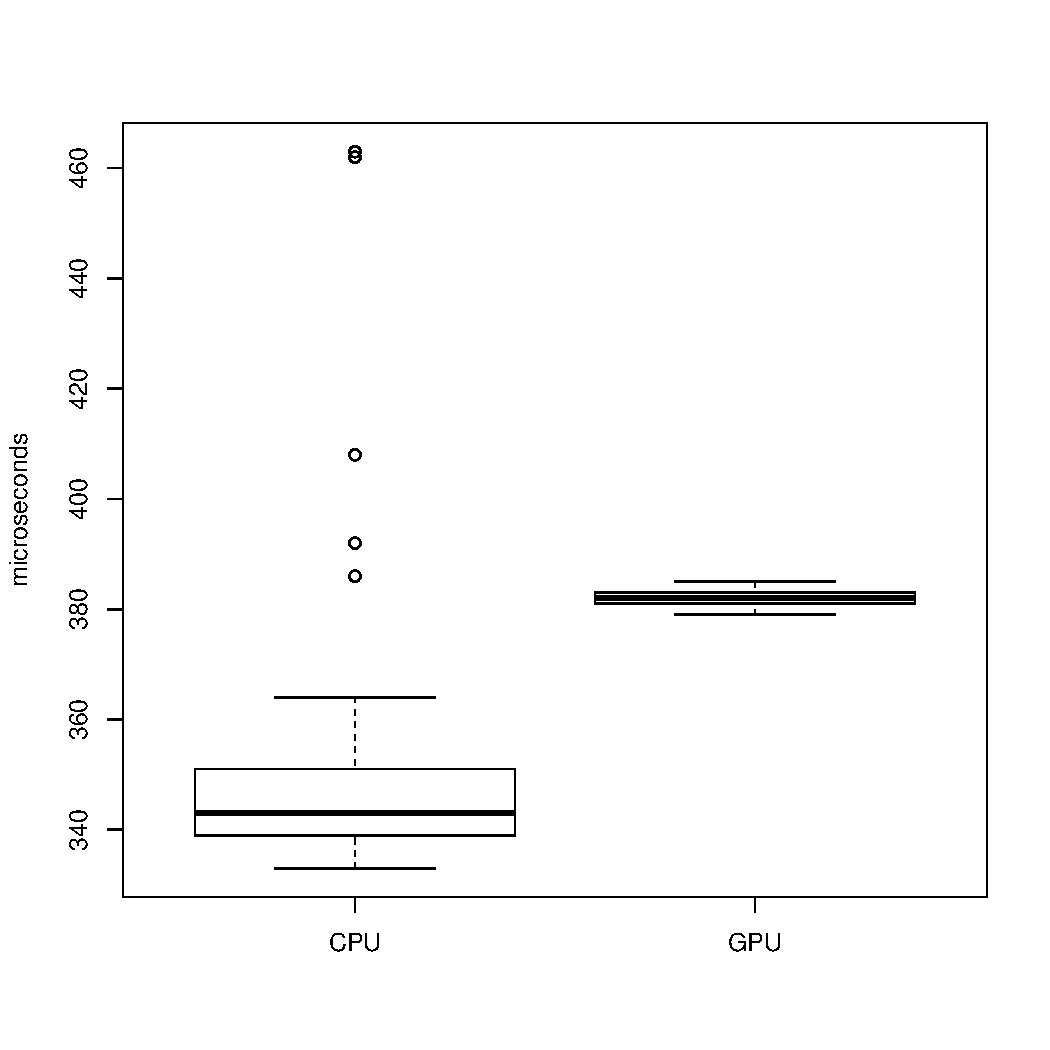
\includegraphics[width=\textwidth]{results/armadillo}
			\caption{Model \texttt{armadillo_10000.txt}}
		\end{subfigure}
		~%
		\begin{subfigure}[b]{0.45\textwidth}
			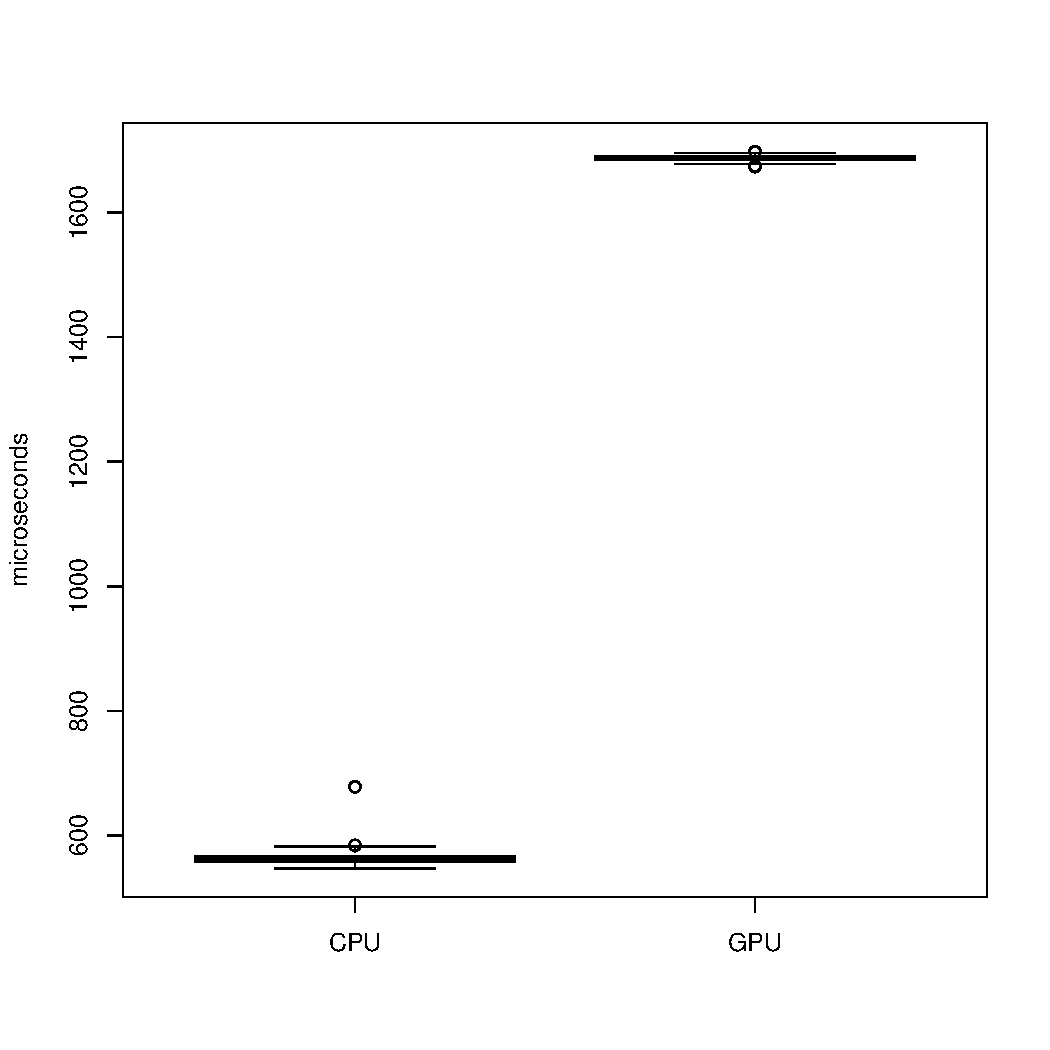
\includegraphics[width=\textwidth]{results/asiandragon9a_50000}
			\caption{Model \texttt{asiandragon9a\_50000.txt}}
		\end{subfigure}
		
		\begin{subfigure}[b]{0.45\textwidth}
			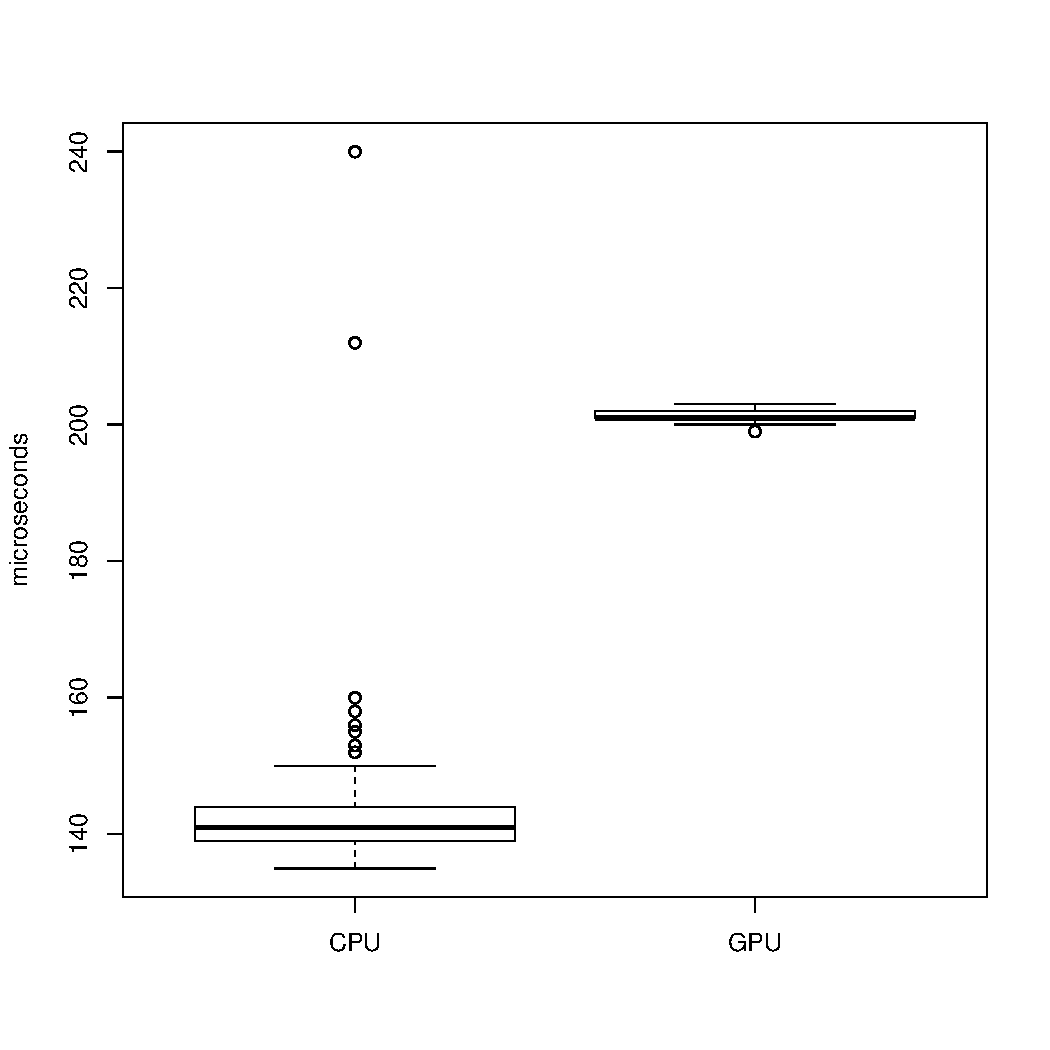
\includegraphics[width=\textwidth]{results/bunny}
			\caption{Model \texttt{bunny.txt}}
		\end{subfigure}
		\label{fig:results}
	\end{figure}
	\begin{figure}
		\ContinuedFloat
		\center
		\begin{subfigure}[b]{0.45\textwidth}
			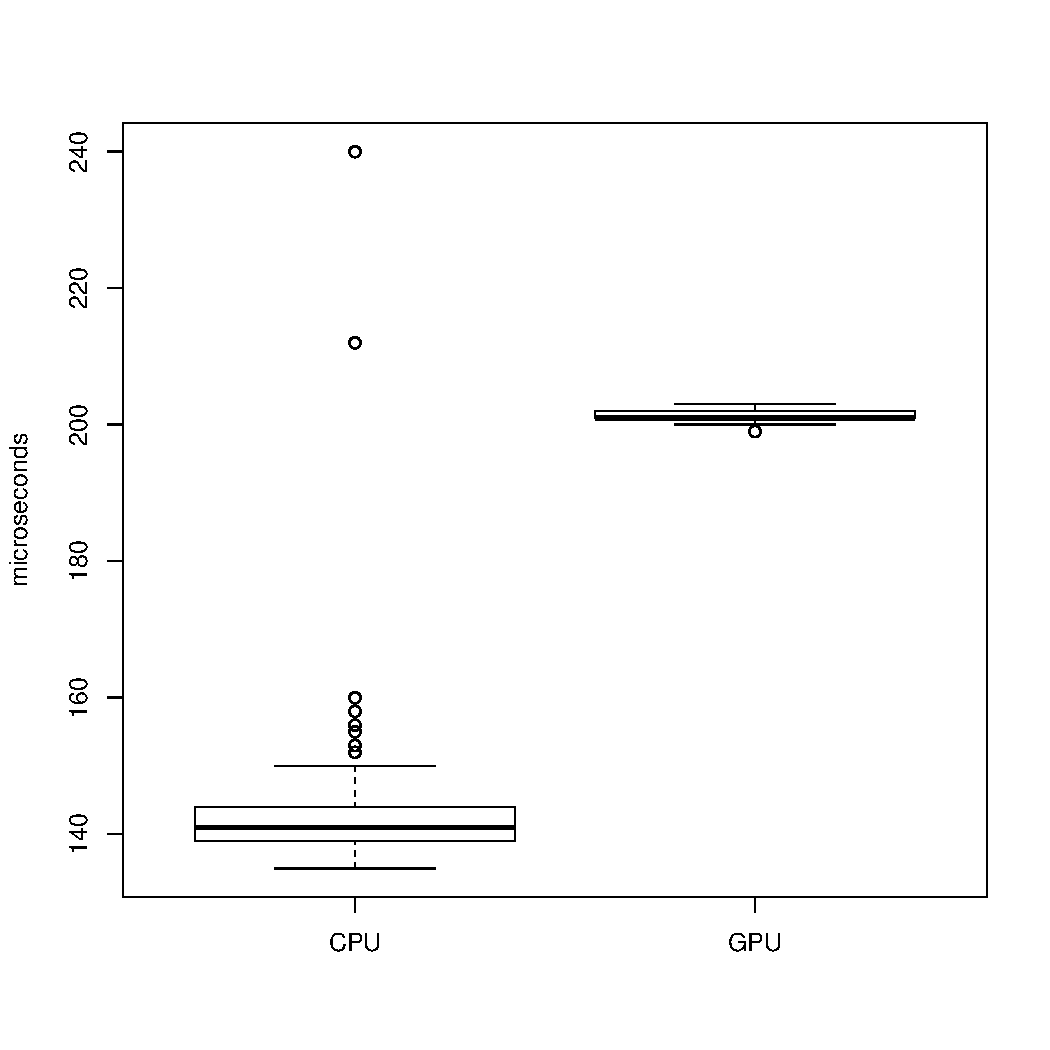
\includegraphics[width=\textwidth]{results/bunny}
			\caption{Model \texttt{bunny2.txt}}
		\end{subfigure}
		\caption{Comparison of CPU and GPU versions}
		~%
		\begin{subfigure}[b]{0.45\textwidth}
			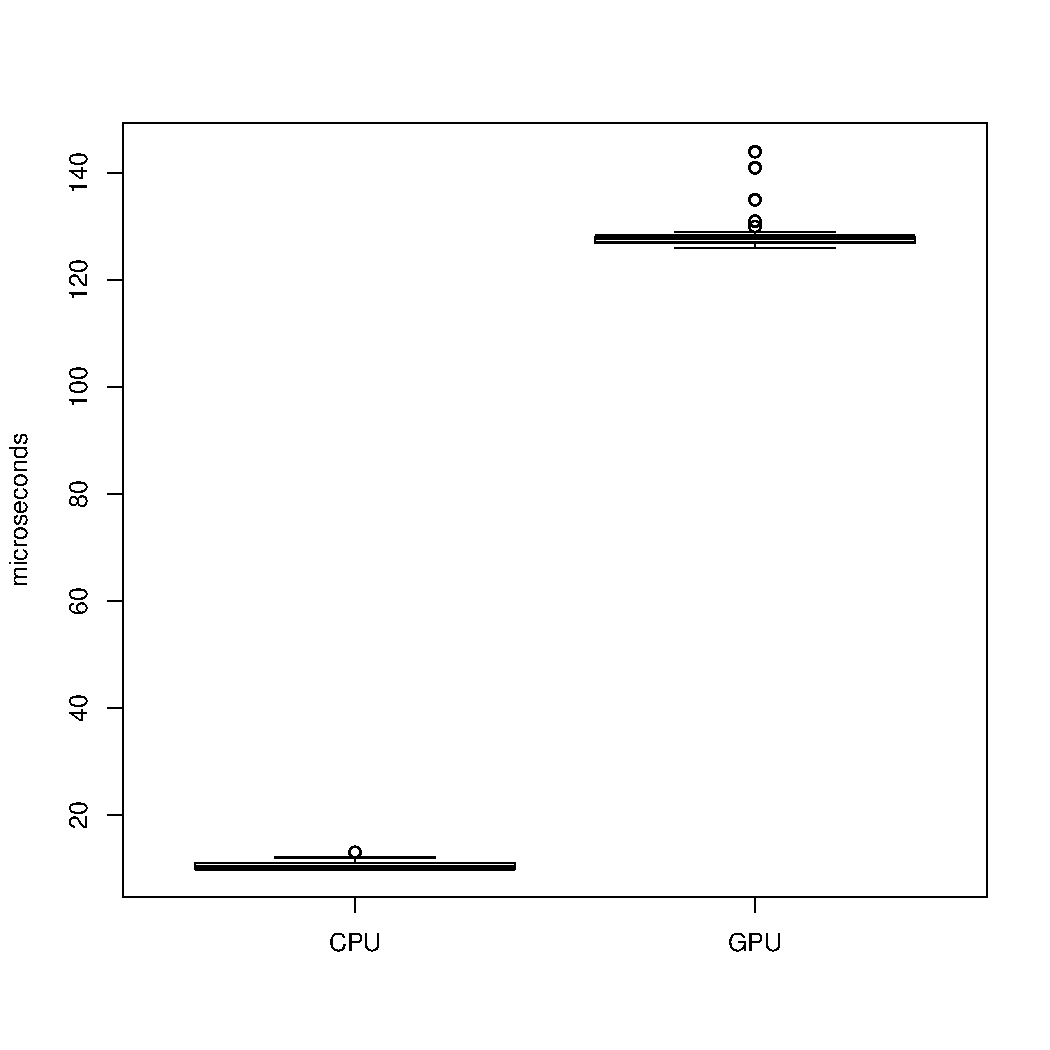
\includegraphics[width=\textwidth]{results/sphere_4000}
			\caption{Model \texttt{sphere\_4000.txt}}
		\end{subfigure}
		\caption[]{Comparison of CPU and GPU versions}
		\label{fig:results}
	\end{figure}
